\documentclass[]{article}
\usepackage{nomencl}
\usepackage{hyperref}
\hypersetup{pdffitwindow=true,
	pdfpagemode=UseThumbs,
	breaklinks=true,
	colorlinks=true,
	linkcolor=black,
	citecolor=black,
	filecolor=black,
	urlcolor=black}

\usepackage{verbatim}
\usepackage[T1]{fontenc}
\usepackage{graphicx}%
\usepackage{amsmath}
\usepackage{amssymb}
\usepackage{amsthm}
\usepackage{subfigure}
\usepackage[makeroom]{cancel}
\usepackage{indentfirst}
\usepackage{color}
\usepackage{bm}
\usepackage{mathtools}

\usepackage{rotating}
\usepackage{comment}
\usepackage{here}
\usepackage{tabularx}
\usepackage{multirow}
\usepackage{setspace}
\usepackage{pdfpages}
\usepackage{float}
\usepackage[section]{placeins}

\usepackage{array}

% quotes
\newcommand{\quotes}[1]{``#1''}

% vectors and such
\newcommand{\vb}[1]{\bm{#1}} % bold
\newcommand{\vbd}[1]{\dot{\bm{#1}}} % dot
\newcommand{\vbdd}[1]{\ddot{\bm{#1}}} % double dot
\newcommand{\vbh}[1]{\hat{\bm{#1}}} % hat
\newcommand{\vbt}[1]{\tilde{\bm{#1}}} % tilde
\newcommand{\vbth}[1]{\hat{\tilde{\bm{#1}}}} % tilde hat
\newcommand{\ddt}[1]{\frac{\mathrm{d} #1}{\mathrm{d} t}} % time derivative
\newcommand{\pd}[2]{\frac{\partial #1}{\partial #2}} % partial derivative
\newcommand{\crossmat}[1]{\left\{ {#1} \right\}^{\times}} % crossmat
\newcommand{\xb}[0]{\vb{x}_b}
\newcommand{\xc}[0]{\vb{x}_c}

\newcommand{\vbr}[0]{\vb{r}}
\newcommand{\vbv}[0]{\vb{v}}

\makenomenclature
\makeindex

\graphicspath{{../../../shared_latex_inputs/images}}

%opening
\title{Math Specification for EMTG-182: Constraint in Two-Body-Rotating Reference Frame}
\author{Noble Hatten}

\begin{document}

\maketitle

\begin{abstract}
	This document is a mathematical specification for ticket EMTG-182: a boundary state constraint expressed in a two-body-rotating reference frame (e.g., the restricted three-body problem rotating frame).

\end{abstract}

\tableofcontents

\printnomenclature

%%%%%%%%%%%%%%%%%%%%%%%%%%%%%%%%%%%%%%%%%%%%%%%%%%%%%%%%%%%%%%%%%%%%%%%%%%%%%%%
\section{Scenario Statement}
\label{sec:scenario_statement}
%%%%%%%%%%%%%%%%%%%%%%%%%%%%%%%%%%%%%%%%%%%%%%%%%%%%%%%%%%%%%%%%%%%%%%%%%%%%%%%

The scenario under consideration consists of two EMTG Universe bodies $B_1$ and $B_2$, and a spacecraft $s$. $B_1$ and $B_2$ can be either the central body of the propagation or any body defined in the Universe of the central body. The geometry of the scenario is described as follows:

\begin{itemize}
	\item $\vb{r}$ is the position vector of $s$ with respect to the central body in the inertial frame. This is part of the state vector.
	\item $\vb{v}$ is the inertial velocity vector of $s$ with respect to the central body in the inertial frame. This is part of the state vector.
	\item $\vb{r}_{1}$ is the position vector of $B_1$ with respect to the central body in theinertial frame. This is an explicit function of time only.
	\item $\vb{v}_{1}$ is the inertial velocity vector of $B_1$ with respect to the central body in the inertial frame. This is an explicit function of time only.
	\item $\vb{r}_{2}$ is the position vector of $B_2$ with respect to the central body in the inertial frame. This is an explicit function of time only.
	\item $\vb{v}_{2}$ is the inertial velocity vector of $B_2$ with respect to the central body in the inertial frame. This is an explicit function of time only.
	\item $\vb{r}_{12} = \vb{r}_2 - \vb{r}_1$ is the inertial position vector from $B_1$ to $B_2$ in the inertial frame. This is an explicit function of time only.
	\item $\vb{v}_{12} = \vb{v}_2 - \vb{v}_1$ is the inertial velocity vector of $B_2$ with respect to $B_1$ in the inertial frame. This is an explicit function of time only.
	\item $\vb{r}_{1s} = \vb{r}_s - \vb{r}_1$ is the inertial position vector from $B_1$ to $s$ in the inertial frame.
	\item $\vb{v}_{1s} = \vb{v}_s - \vb{v}_1$ is the inertial velocity vector of $s$ with respect to $B_1$ in the inertial frame.
	\item $\vb{r}_{2s} = \vb{r}_s - \vb{r}_2$ is the inertial position vector from $B_2$ to $s$ in the inertial frame.
	\item $\vb{v}_{2s} = \vb{v}_s - \vb{v}_2$ is the inertial velocity vector of $s$ with respect to $B_2$ in the inertial frame.
	\item $\vb{\omega}$ is the instantaneous angular velocity vector of $B_2$ with respect to $B_1$. This is an explicit function of time only.
\end{itemize}

In practice, the inertial frame is the ICRF.

\nomenclature{$B_1$}{Universe body 1}
\nomenclature{$B_2$}{Universe body 2}
\nomenclature{$s$}{Spacecraft}
\nomenclature{$\vb{r}$}{Position vector of spacecraft $s$ with respect to the central body in the inertial frame}
\nomenclature{$\vb{v}$}{Inertial velocity vector of spacecraft $s$ with respect to the central body in the inertial frame}
\nomenclature{$\vb{r}_1$}{Position vector of body $B_1$ with respect to the central body in the inertial frame}
\nomenclature{$\vb{v}_1$}{Inertial velocity vector of body $B_1$ with respect to the central body in the inertial frame}
\nomenclature{$\vb{r}_2$}{Position vector of body $B_2$ with respect to the central body in the inertial frame}
\nomenclature{$\vb{v}_2$}{Inertial velocity vector of body $B_2$ with respect to the central body in the inertial frame}
\nomenclature{$\vb{r}_{12}$}{Inertial position vector from body $B_1$ to body $B_2$ in the inertial frame}
\nomenclature{$\vb{v}_{12}$}{Inertial velocity vector of body $B_2$ with respect to body $B_1$ in the inertial frame}
\nomenclature{$\vb{r}_{1s}$}{Inertial position vector from body $B_1$ to spacecraft $s$ in the inertial frame}
\nomenclature{$\vb{v}_{1s}$}{Inertial velocity vector of spacecraft $s$ with respect to body $B_1$ in the inertial frame}
\nomenclature{$\vb{r}_{2s}$}{Inertial position vector from body $B_2$ to $s$ in the inertial frame}
\nomenclature{$\vb{v}_{2s}$}{Inertial velocity vector of spacecraft $s$ with respect to body $B_2$ in the inertial frame}
\nomenclature{$\vb{\omega}$}{Instantaneous angular velocity vector of body $B_2$ with respect to body $B_1$}
\nomenclature{$I$}{As a subscript, indicates a vector expressed in the inertial frame. This is the default assumption if no subscript is present.}
\nomenclature{$R$}{As a subscript, indicates a vector expressed in the two-body rotating frame.}

The geometry is displayed graphically in Figure \ref{fig:geometry}.

\begin{figure}
	\centering
	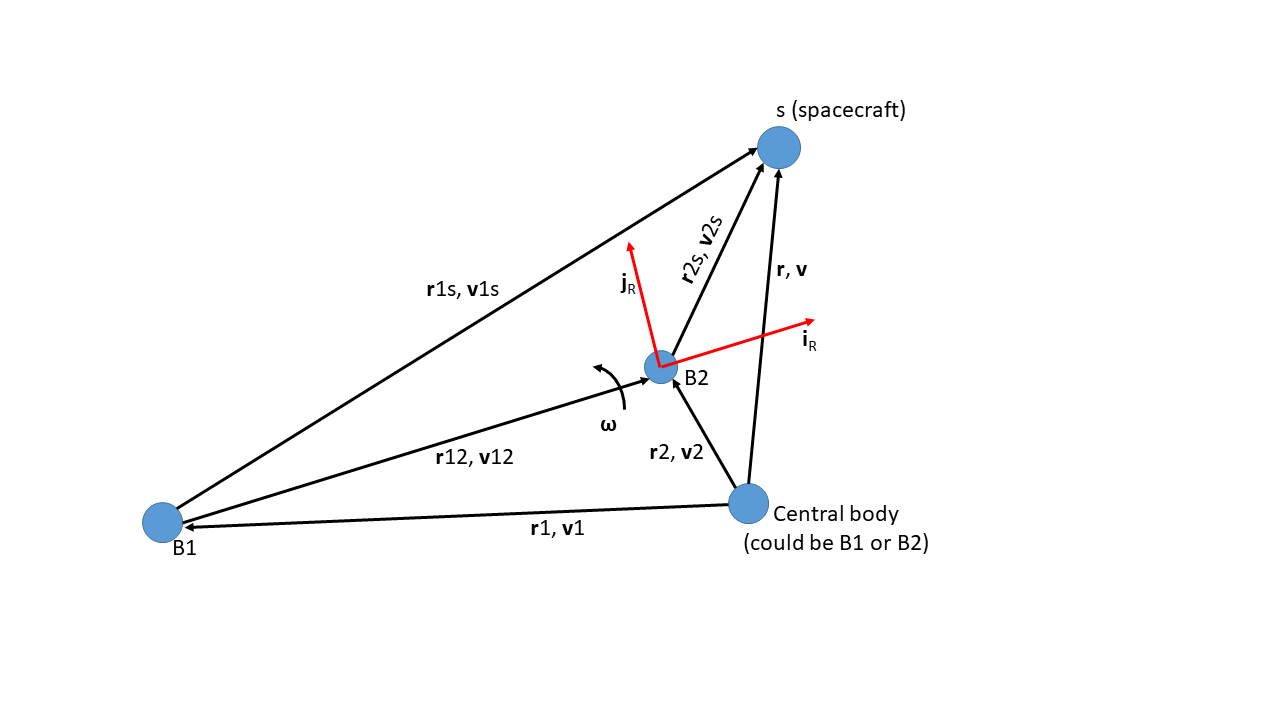
\includegraphics[trim=1.5in 1.5in 4.25in 4.0in, width=.88\linewidth]{constraint_in_two_body_frame_geometry2.PNG}
	%\captionsetup{justification=centering}
	\caption{Geometry of the scenario.}
	\label{fig:geometry}
\end{figure}

%%%%%%%%%%%%%%%%%%%%%%%%%%%%%%%%%%%%%%%%%%%%%%%%%%%%%%%%%%%%%%%%%%%%%%%%%%%%%%%
\section{Two-Body Rotating Frame}
\label{sec:two_body_rotating_frame}
%%%%%%%%%%%%%%%%%%%%%%%%%%%%%%%%%%%%%%%%%%%%%%%%%%%%%%%%%%%%%%%%%%%%%%%%%%%%%%%

The two-body rotating frame is defined such that the origin is coincident with $B_2$, and the axes are:

\begin{itemize}
	\item $\vbh{i}_R = \vbh{r}_{12}$
	\item $\vbh{k}_R = \vbh{\omega}$
	\item $\vbh{j}_R$ completes the right-handed set. I.e., $\vbh{j}_R = \vbh{k}_R \times \vbh{i}_R$.
\end{itemize}

\noindent A subscript $R$ is used to indicate that a vector is expressed in the two-body rotating frame.

\nomenclature{$\vb{r}_{2s, R}$}{Position vector from $B_2$ to $s$ expressed in the two-body rotating frame}
\nomenclature{$\vb{v}_{2s, R}$}{Velocity vector of $s$ with respect to $B_2$ expressed in the two-body rotating frame}

%%%%%%%%%%%%%%%%%%%%%%%%%%%%%%%%%%%%%%%%%%%%%%%%%%%%%%%%%%%%%%%%%%%%%%%%%%%%%%%
\subsection{Angular Velocity of Body 2 with Respect to Body 1}
\label{sec:angular_velocity}
%%%%%%%%%%%%%%%%%%%%%%%%%%%%%%%%%%%%%%%%%%%%%%%%%%%%%%%%%%%%%%%%%%%%%%%%%%%%%%%

The magnitude of the angular velocity is the time derivative of the angular displacement of $B_2$ about $B_1$, and the direction of the angular velocity vector is in the direction of the angular momentum of $B_2$ about $B_1$. For brevity, redefine $\vb{r} \triangleq \vb{r}_{12}$ and $\vb{v} \triangleq \vb{v}_{12}$ in this section only for the purposes of this derivation.

Common knowledge:

\begin{align}
\dot{\nu} &= \frac{h}{r^2} \\
\vb{h} &= \vb{r} \times \vb{v}
\end{align}

\nomenclature{$\vb{h}$}{Specific orbital angular momentum vector}

\noindent So:

\begin{align}
\vb{\omega} &= \dot{\nu} \vbh{h} \\
&= \frac{h}{r^2} \frac{\vb{h}}{h} \\
&= r^{-2} \vb{h} \\
&= r^{-2} \left( \vb{r} \times \vb{v} \right)
\end{align}

We also require the derivatives of $\vb{\omega}$. $\vb{\omega}$ is an explicit function of time only because it only depends on the positions and velocities of $B_1$ and $B_2$, which are ephemeris lookups.

\begin{align}
\ddt{\vb{\omega}} &= \ddt{\left( r^{-2} \vb{h} \right)} \\
&= \ddt{r^{-2}} \vb{h} + r^{-2} \ddt{\vb{h}}
\end{align}

\noindent Then:

\begin{align}
\ddt{r^{-2}} &= -2 r^{-3} \ddt{r} \\
\ddt{r} &= \pd{r}{\vb{r}} \ddt{\vbr} \\
&= \frac{\vb{r}^T}{r} \ddt{\vbr} \\
\rightarrow \ddt{r^{-2}} &= \frac{-2}{r^4} \vb{r}^T \ddt{\vbr}
\end{align}

\noindent Important note: $\vbv$ is not substituted for $\ddt{\vbr}$ here because these two quantities are not necessarily equal, depending on how the ephemeris is implemented.

We also have

\begin{align}
\ddt{\vb{h}} &= \pd{\vb{h}}{\vb{r}} \ddt{\vbr} + \pd{\vb{h}}{\vb{v}} \ddt{\vbv}
\end{align}

\noindent where:

\begin{align}
\pd{\vb{h}}{\vb{r}} &= -\crossmat{\vb{v}} \\
\pd{\vb{h}}{\vb{v}} &= \crossmat{\vb{r}} \\
\end{align}

\noindent Like $\vb{r}$ and $\vb{v}$, $\ddt{\vbr}$ and $\ddt{\vbv}$ are ephemeris lookups. Again, note that $\vb{v}$ is not substituted for $\ddt{\vbr}$.

%%%%%%%%%%%%%%%%%%%%%%%%%%%%%%%%%%%%%%%%%%%%%%%%%%%%%%%%%%%%%%%%%%%%%%%%%%%%%%%
\subsection{Transformation from ICRF to Two-Body Rotating Frame}
\label{sec:icrf_to_two_body_rotating_frame}
%%%%%%%%%%%%%%%%%%%%%%%%%%%%%%%%%%%%%%%%%%%%%%%%%%%%%%%%%%%%%%%%%%%%%%%%%%%%%%%

To express a generic vector given in frame $I$ in the two-body rotating frame $R$, we have

\begin{align}
\label{eq:transformation_matrix}
\vb{r}_{R} &= \vb{R}^{I \rightarrow R} \vb{r}_{I}
\end{align}

\noindent From the dot product definition of the direction cosine matrix, we get

\begin{align}
\vb{R}^{I \rightarrow R} &= \left[ \vbh{i}_R \quad\vbh{j}_R \quad \vbh{k}_R \right]^T,
\end{align}

\noindent where the unit vectors are defined in Section~\ref{sec:two_body_rotating_frame} and the quantities expressed in the $I$ frame.

%%%%%%%%%%%%%%%%%%%%%%%%%%%%%%%%%%%%%%%%%%%%%%%%%%%%%%%%%%%%%%%%%%%%%%%%%%%%%%%
\subsubsection{Time Derivative of Transformation Matrix}
\label{sec:time_derivative_of_transformation_matrix}
%%%%%%%%%%%%%%%%%%%%%%%%%%%%%%%%%%%%%%%%%%%%%%%%%%%%%%%%%%%%%%%%%%%%%%%%%%%%%%%

The time derivative of $\vb{R}^{I \rightarrow R}$ is obtained by differentiating the unit vectors of the rotating frame with respect to time.

\begin{align}
	\dot{\vbh{i}}_R &= \pd{\vbh{i}_R}{\vbr_{12}} \ddt{\vbr_{12}}
\end{align}

\noindent $\ddt{\vbr_{12}}$ is an ephemeris lookup (but not $\vbv_{12}$!). Since $\vbh{i}_R = \vbh{r}_{12}$, we use the well-known derivative of a unit vector with respect to its non-unitized vector:

\begin{align}
	\pd{\vbh{r}_{12}}{\vbr_{12}} &= \frac{1}{r_{12}} \left( \vb{I} - \frac{1}{r_{12}^2} \vb{r}_{12} \vb{r}_{12}^T \right)
\end{align}

$\dot{\vbh{k}}_R$ is similar.

\begin{align}
\dot{\vbh{k}}_R &= \pd{\vbh{k}_R}{\vb{\omega}} \ddt{\vb{\omega}} \\
&= \frac{1}{\omega} \left( \vb{I} - \frac{1}{\omega^2} \vb{\omega} \vb{\omega}^T \right) \ddt{\vb{\omega}}
\end{align}

\noindent $\ddt{\vb{\omega}}$ is obtained from the equations in Section~\ref{sec:angular_velocity}.

For $\dot{\vbh{j}}_R$, we can use

\begin{align}
	\dot{\vbh{j}}_R &= \pd{\vbh{j}_R}{\vbh{i}_R} \dot{\vbh{i}}_R + \pd{\vbh{j}_R}{\vbh{k}_R} \dot{\vbh{k}}_R
\end{align}

\noindent Since $\vbh{j}_R = \vbh{k}_R \times \vbh{i}_R$,

\begin{align}
	\pd{\vbh{j}_R}{\vbh{i}_R} &= \crossmat{\vbh{k}_R} \\
	\pd{\vbh{j}_R}{\vbh{k}_R} &= -\crossmat{\vbh{i}_R}
\end{align}

%%%%%%%%%%%%%%%%%%%%%%%%%%%%%%%%%%%%%%%%%%%%%%%%%%%%%%%%%%%%%%%%%%%%%%%%%%%%%%%
\subsubsection{Position with Respect to Body 2}
\label{sec:position_wrt_body2}
%%%%%%%%%%%%%%%%%%%%%%%%%%%%%%%%%%%%%%%%%%%%%%%%%%%%%%%%%%%%%%%%%%%%%%%%%%%%%%%

The specific position quantity we wish to constrain is the position of the spacecraft relative to Body 2, expressed in the rotating frame: $\vbr_{2s, R}$. Using Eq.~\eqref{eq:transformation_matrix}, we have

\begin{align}
	\vb{r}_{2s, R} &= \vb{R}^{I \rightarrow R} \vb{r}_{2s,I} \\
	&= \vb{R}^{I \rightarrow R} \left( \vbr_{s,I} - \vbr_{2,I} \right)
\end{align}

\noindent $\vbr_{s,I}$ is made up only of elements of the state vector (i.e., it is not an explicit function of time), while $\vbr_{2,I}$ is \emph{only} a function of time. We require the derivatives of $\vb{r}_{2s, R}$ with respect of our independent variables. The relevant independent variables are the position state $\vbr_{s,I}$ and time $t$. Differentiating with respect to $\vbr_{s,I}$ gives

\begin{align}
	\pd{\vb{r}_{2s, R}}{\vbr_{s,I}} &= \vb{R}^{I \rightarrow R}
\end{align}

\noindent Differentiating with respect to $t$ gives

\begin{align}
	\label{eq:dr2srdt}
	\pd{\vb{r}_{2s, R}}{t} &= \vbd{R}^{I \rightarrow R} \vbr_{s,I} - \left[ \vbd{R}^{I \rightarrow R} \vbr_{2,I} + \vb{R}^{I \rightarrow R} \ddt{\vbr_{2,I}} \right]
\end{align}

\noindent All elements of Eq.~\eqref{eq:dr2srdt} except $\vbr_{s,I}$ are explicit functions of time only. $\ddt{\vbr_{2,I}}$ is obtained from ephemeris lookups. $\vbd{R}^{I \rightarrow R}$ is obtained by differentiating the unit vectors of the rotating frame with respect to time.

%%%%%%%%%%%%%%%%%%%%%%%%%%%%%%%%%%%%%%%%%%%%%%%%%%%%%%%%%%%%%%%%%%%%%%%%%%%%%%%
\subsubsection{Velocity with Respect to Body 2}
\label{sec:velocity_wrt_body2}
%%%%%%%%%%%%%%%%%%%%%%%%%%%%%%%%%%%%%%%%%%%%%%%%%%%%%%%%%%%%%%%%%%%%%%%%%%%%%%%

For the velocity vector, we must differentiate, in the colloquial sense, between velocities relative to the inertial frame and the rotating frame. This difference is denoted with a preceding superscript: $I$ indicates the derivative is taken with respect to the inertial frame, and $R$ indicates that the derivative is taken with respect to the rotating frame.

The velocity of the spacecraft relative to the rotating frame centered at $B_2$, expressed in the inertial frame, is

\begin{align}
	{}^R \vbv_{2s,I} &= {}^I \vbv_{2s,I} - \vb{\omega}_I \times \vbr_{2s,I}
\end{align}

\noindent We wish to express this velocity in the rotating frame, so we use our transformation matrix:

\begin{align}
{}^R \vbv_{2s,R} &= \vb{R}^{I \rightarrow R} \left( {}^I \vbv_{2s,I} - \vb{\omega}_I \times \vbr_{2s,I} \right)
\end{align}


We also require the derivatives of ${}^R \vb{v}_{2s}$. ${}^R \vb{v}_{2s}$ depends on both time and on the spacecraft state.

The derivative of ${}^R \vb{v}_{2s,R}$ with respect to an arbitrary variable $x$ is

\begin{align}
	\label{eq:dvr2s_top_level}
	\pd{{}^R \vb{v}_{2s,R}}{x} &= \pd{\vb{R}^{I \rightarrow R}}{x} \left( {}^I \vbv_{2s,I} - \vb{\omega}_I \times \vbr_{2s,I} \right) + \vb{R}^{I \rightarrow R} \pd{ \left( {}^I \vbv_{2s,I} - \vb{\omega}_I \times \vbr_{2s,I} \right)}{x}
\end{align}

\noindent As before, the derivatives of $\vb{R}^{I \rightarrow R}$ is obtained by differentiating the unit vectors of the rotating frame with respect to time. $\vb{R}^{I \rightarrow R}$ depends only on the location of $B_2$ with respect to $B_1$ and is therefore a function of time only. As a result, $\pd{\vb{R}^{I \rightarrow R}}{x}$ is obtained from ephemeris lookups if $x = t$ and 0 otherwise.

For the second term on the right-hand side of Eq.~\ref{eq:dvr2s_top_level}, we obtain

\begin{align}
	\pd{ \left( {}^I \vbv_{2s,I} - \vb{\omega}_I \times \vbr_{2s,I} \right)}{x} &= \pd{ \left( {}^I \vbv_{2s,I} \right)}{x} - \pd{ \left(\vb{\omega}_I \times \vbr_{2s,I} \right)}{x}
\end{align}

\noindent where

\begin{align}
\pd{\left({}^I \vbv_{2s,I} \right)}{x} &= \pd{\left({}^I \vbv_{s,I} \right)}{x} - \pd{\left({}^I \vbv_{2,I} \right)}{x} 
\end{align}

\noindent in which $\pd{\left({}^I \vbv_{s,I} \right)}{x} = \vb{I}$ if $x = {}^I \vbv_{s,I}$ and is $0$ otherwise. $ \pd{\left({}^I \vbv_{2,s} \right)}{x}$ is an ephemeris lookup ($\dot{\vbv}_2$) if $x = t$ and is $0$ otherwise.

Finally,

\begin{align}
	\pd{\left( \vb{\omega}_I \times \vbr_{2s,I} \right)}{x} &= \pd{\left( \vb{\omega}_I \times \vbr_{2s,I} \right)}{\vb{\omega}_I} \pd{\vb{\omega}_I}{x} + \pd{\left( \vb{\omega}_I \times \vbr_{2s,I} \right)}{\vbr_{2s,I}} \pd{\vbr_{2s,I}}{x} \\
	\pd{\left( \vb{\omega}_I \times \vbr_{2s,I} \right)}{\vb{\omega}_I} &= - \crossmat{\vbr_{2s,I}} \\
	\pd{\left( \vb{\omega}_I \times \vbr_{2s,I} \right)}{\vbr_{2s,I}} &= \crossmat{\vb{\omega}_I} \\
	\pd{\vbr_{2s,I}}{x} &= \pd{\vbr_{s,I}}{x} - \pd{\vbr_{2,I}}{x}
\end{align}

\noindent $\pd{\vb{\omega}_I}{x}$ is given in Section~\ref{sec:angular_velocity} if $x = t$ and is $0$ otherwise. $\pd{\vbr_{s,I}}{x} = \vb{I}$ if $x = \vb{r}_{s,I}$ (part of the state vector) and $0$ otherwise. $\pd{\vbr_{2,I}}{x}$ is an ephemeris lookup ($\ddt{\vbr_{2,I}}$) if $x = t$ (an ephemeris lookup) and $0$ otherwise.

%\bibliography{}
%\bibliographystyle{plain}

\end{document}